%%%%%%%%%%%%%%%%%%%%%%%%%%%%%%%%%%%%%%%%%%%%%%%%%%%%%%%%%%%%%%%%%%%%%%
%%%  Semantic technologies for Airbus use case%%%%
%%%%%%%%%%%%%%%%%%%%%%%%%%%%%%%%%%%%%%%%%%%%%%%%%%%%%%%%%%%%%%%%%%%%%%

\documentclass[runningheads,a4paper]{{llncs}}

\usepackage[utf8]{inputenc}
\usepackage{amssymb}
\setcounter{tocdepth}{3}
\usepackage{graphicx}
\usepackage{tabularx}
\usepackage{url}
\usepackage{listings}
\usepackage{subfigure}
\usepackage{algorithm,algorithmic}
\usepackage{cleveref}
\usepackage{xcolor}
\usepackage{pifont}
\usepackage{multirow}

\newcommand{\keywords}[1]{\par\addvspace\baselineskip
\noindent\keywordname\enspace\ignorespaces#1}
% defining checklist in item
\newcommand{\myitem}{\item[\checkmark]}
%defining xmark in item
\newcommand{\xmark}{\ding{55}}
\newcommand{\xitem}{\item[\xmark]}

% todo macro
\usepackage{color}
\newtheorem{deflda}{Axiom}
\newcommand{\todo}[1]{\noindent\textcolor{red}{{\bf \{TODO}: #1{\bf \}}}}

% Language Definitions for Turtle
\definecolor{olivegreen}{rgb}{0.2,0.8,0.5}
\definecolor{grey}{rgb}{0.5,0.5,0.5}
\definecolor{background}{HTML}{EEEEEE}

\lstdefinelanguage{ttl}{
sensitive=true,
morecomment=[l][\color{brown}]{@},
morecomment=[l][\color{red}]{\#},
morestring=[b][\color{blue}]\",
}

\lstdefinelanguage{turtle}
{
    columns=fullflexible,
    keywordstyle=\color{red},
    morekeywords={PREFIX,SELECT,DISTINCT,UNION,FILTER,ORDER,BY,REGEX,STR,STRSTARTS,GRAPH,isBlank},
    morecomment=[l]{\#},
    tabsize=4,
    frame=lines,
    numbers=left,
    numberfirstline=true,
    xleftmargin=2.5em,
    framexleftmargin=2.8em,
    stepnumber=1,    
    firstnumber=1,
    alsoletter={-?}, % allowed in names
    morecomment=[s][\color{blue}]{<}{>},
    commentstyle=\color{green!40!black},
    basicstyle=\scriptsize\ttfamily\color{black},
    %numberstyle=\color{black},
    morestring=[b][\color{black}]\",
    backgroundcolor=\color{background},    
    showstringspaces=false
}
%%%%%%%%%%%%%%%%%%%%%%%%%%%%%%%
%%%  Beginning of document  %%%
%%%%%%%%%%%%%%%%%%%%%%%%%%%%%%%

\begin{document}


%\title{Semantic Technologies for Matching Operational Interruptions to Tasks in Aircraft Industry }
%\title{Assessing Operational Interruptions in Aircraft Industry With Semantic Technologies: A Use-Case at Airbus}
\title{Semantic Annotation and Matching of Operational Interruptions in Aircraft Industry: A Use-Case at Airbus}
%\subtitle{Classifying vocabularies }

\author{ Ghislain Auguste Atemezing\inst{1}, Dang Nguyen-manh\inst{2} }

\institute{
MONDECA, 35 Boulevard de Strasbourg, Paris, France. \\
\and Airbus, Toulouse, France.\\
\email{ghislain.atemezing@mondeca.com} \\
\email{dang.nguyeng-manh@airbus.com} \\
}
  


% a short form should be given in case it is too long for the running head
\titlerunning{Semantics Applied to Detecting OIs in Aircraft Industry}	


\maketitle

%%%%%%%%%%%%%%%%%%
%%%  Abstract  %%%
%%%%%%%%%%%%%%%%%%

\begin{abstract}

Airbus, one of the leading Aircraft company in Europe, collects and manages a substantial amount of unstructured data from airlines companies, related to events occurring during the exploitation of an aircraft. Those events are called ``Operational Interruptions'' (OI) describing observations and the work performed associated by operators in form of short text. At the same time, Airbus maintains a dataset of programmed maintenance task (MPD) for each family of aircraft.  Currently, OIs are reported by companies  in Excel spreadsheets and experts have to find manually in the OIs the ones that are most likely to match an existing task. In this paper, we describe a semi-automatic approach using semantic technologies to assist the experts of the domain to improve the matching process of OIs with related MPD. Our approach combines text annotation using GATE and a graph matching algorithm. The evaluation of the approach shows the benefits of using semantic technologies to manage unstructured data and future applications for data integration at Airbus.    

\keywords{Information Retrieval, tagging system, Graph matching, CA-Manager, GATE, Airbus}
\end{abstract}

%%%%%%%%%%%%%%%%%%%%%%%%%
%%%  1. Introduction  %%%
%%%%%%%%%%%%%%%%%%%%%%%%%

\section{Introduction}
\label{sec:introduction}
Semantics enable machine-to-machine exchange and automated processing of data to facilitate the integration of business processes and systems~\cite{cardoso2007}. The main goal of having machine readable information is to search, reuse information and develop innovative applications easier. 
Semantic Web~\cite{berners2001} technologies are becoming more and more adopted outside the research communities or academics. The most promising of adopting these technologies is the benefits of using open standards developed by the W3C. Linked (open) data~\cite{bizer2009} has already shown its application in many domains, such as health, cultural heritage, libraries, etc. What is starting to appear is the use of semantics in aircraft industries where some often tools developed by the semantic web are perceived to be not mature enough by expert domains. This paper describes the challenges of using semantic technologies for matching events occurred during the exploitation of an aircraft reported by a company with the official list of maintenance programmed by Airbus during the life-cycle of a given aircraft. The goal is to update the maintenance task (MPD) with new issues if the detection of operational interruptions (OIs) is relevant. The ultimate goal is to anticipate failures reported by the aircraft companies to the manufacturer. The main contributions of this paper are the following: (i) Capture the implicit knowledge of expert domains in RDF for generating gazetteers using SKOS~\cite{skosw3c} concepts;  (ii) propose and implement a semantic annotation workflow to detect relevant OIs concepts and (iii) implement a robust graph matching algorithm to make recommendation to expert for assessment and validation. The results obtained are very promising as we are able to obtain a high level detected OIs (81.52\%) with a very limited amount of keywords provided by experts (less than 150 concepts in the gazetteer). The paper is structured as follow: In Section~\ref{sec:statement}, an overview of the domain expertise and problem statement are presented, followed by the vocabularies and data model in Section~\ref{sec:data-model}. Section~\ref{sec:a330rdf} describes the dataset converted in RDF. The semantic annotation is described in Section~\ref{sec:annotation}, then the graph matching algorithm is presented in Section~\ref{sec:matching}. The experiments and lessons learned are respectively presented in Section~\ref{sec:exp-results} and Section~\ref{sec:lessons}. Section~\ref{sec:soa} briefly expose some related work before concluding of the paper.    

%\todo{Show the problem and implication}



\section{Problem Statement}
\label{sec:statement}
In this section, we describe the scope of the domain at Aircraft and the main challenge of the provided solution in this paper. We first describe the concepts related to aircraft domain of our study, and then presents the approach using semantic technologies to tackle this real-world use-case.

\subsection{Domain Description}
Operational interruptions (OIs) are incidents occurring during the use of the aircraft, with an impact on commercial exploitation. All maintenance events are not OIs though: we need a minimal delay time for this to be considered an OI, i.e., if the cause is neutralized very quickly, an OI is not generated). Secondly, the OIs are not only technical incidents due to an aircraft: a crew arriving late because the van had broken down can also be an OI. Also, some elements occurring in the plane does not have a "technical" cause: for example, a collision with a bird (bird strike) will require maintenance, while the plane itself was not involved.

Generally, an OI contains the description of the interruption (what happened: it may be an effect or failure (failure message, vibration, noise, etc.) or a description of what the pilots or ground personnel observed), actions taken to address them (sometimes there are none), and additional metadata as the ATA code~\footnote{\url{https://en.wikipedia.org/wiki/ATA_100}}, the aircraft (type, operator, number, engine, etc) the ``changeability'' (e.g., is it due to the plane? to ground maintenance teams? etc), the operational impact (does that re-routed the plane? Did that cancel the flight? etc), the type of failure, etc. Today, OIs are used primarily for teams studying aircraft reliability to derive statistics and make recommendations. 

Scheduled maintenance aims to avoid preemptively that some outages occur, develop into silence and ultimately have a significant impact on the use of the aircraft or its security. Some tasks are performed ``before'' the effect occurs: inspection of areas, equipment testing, periodic replacement.
Not all parts of the aircraft are subject to scheduled maintenance. For example, some devices have sensors, integrated testing means, and thus emit messages in case of failure or when their condition deteriorates - so they perform in these cases, corrective maintenance. Therefore, many OIs concern elements that scheduled maintenance would not have prevented.

Scheduled maintenance tasks are described in the Maintenance Planning Document (MPD), with their title, interval, the areas where they occur, the necessary duration, etc. However, the MPD itself does not describe why it is necessary to perform these tasks.


The Maintenance Review Board Report (MRBR) falls under analysis by experts of scheduled maintenance, in agreement with the authorities and operators. The objective of these teams is to see if the items to be covered are often detected or not, to adjust the range of preventive actions to more suitable ones. Therefore, they look at reports of scheduled maintenance operations (reports of "Findings"), but need also data from non-scheduled operations to be complete: which require the analysis of OIs.

Each MRBR item is a task involving one or more functions, each of which can have multiple causes, which will induce a functional failure in systems of the plane, which will have effects or consequences on the plane (detectable or not). Each row in the MRBR describes a failure. A link exists between MRBR and MPD task: each MPD task can cover one or more MRBR items(or none) some MPD tasks are derived from further analysis. 


This paper solves the following challenge: identify the indirect link between OI and MPD task. That is: if the IO describes a cause that would have been avoided by conducting an MPD task, then we associate the corresponding MPD task. Therefore, we seek in OI (description, metadata), if there are elements related to potentially preventable failures of MPD, so as to associate it causes, failures and consequences described in MRBR items. Hence the keywords used by experts to identify potentially interesting OI.

\subsection{Our Approach}
\label{sec:approach}
The main challenge is to assist the expert with a reduced list of OIs candidates that can be matched with some existing tasks in the MPD. The top down approach takes a task, uses the list of keywords and the implicit knowledge of the expert (e.g., experience) and try to match with OI. Currently this is the approach manually used by domain experts by means of formulas in spreadsheets to find and filter sets of OIs based on list of keywords. A second approach consisting a fully automatic process, from OIs annotations and matching without experts in the loop (bottom-up approach) was not acceptable by the domain experts. We define an \textit{hybrid approach} where the expert can assess and validate the results of the approach, consisting of the following (as shown in Figure~\ref{fig:approach}):
\begin{enumerate}
\item OIs are annotated with keywords from the experts.
\item MP tasks already treated are modeled in RDF with associated keywords.
\item Find OIs candidates matching the set of reference tasks by using any relevance information such as ATA references and aircraft metadata.
\item Experts evaluate and validate the suggested OIs candidates.
\end{enumerate}  

\begin{figure}[!htb]
\centering
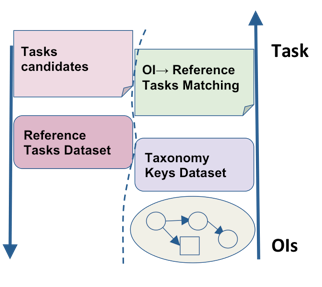
\includegraphics[scale=0.6]{img/ourapproach.png}
\caption{The hybrid approach used to match the OI descriptions with MPD tasks, using semantic technologies.}
\label{fig:approach}
\end{figure}


\section{Vocabularies and Data Model}
\label{sec:data-model}
The legacy data in spreadsheets is converted into RDF for better integration and homogeneity. Two vocabularies is designed to capture the knowledge presented in the diverse data: a vocabulary for operational interruptions (oi-vocab) and a vocabulary for maintenance tasks and analysis experts report (task-vocab). The URI namespaces used for the vocabularies follow the pattern \textit{http://data.airbus.com/def/\{vocab-prefix\}\#}. 

\subsection{OI vocabulary}
\label{oivocab}
The OI vocabulary\footnote{\url{http://data.airbus.com/def/oi#}} is a lightweight model with one main class and three data properties. An operational interruption is modeled as a subclass of an event, reusing the class \textsf{event:Event} of the event ontology\footnote{\url{http://purl.org/NET/c4dm/event.owl}}. The data properties \textsf{oi:ataref}, \textsf{oi:description} and \textsf{oi:workPerform} are used to respectively capture the ATA reference, the textual description of an OI and the work performed by an operator. Figure~\ref{figoi} depicts the vocabulary and a sample graph generated with the model. 

\begin{figure}[!htb]
\centering
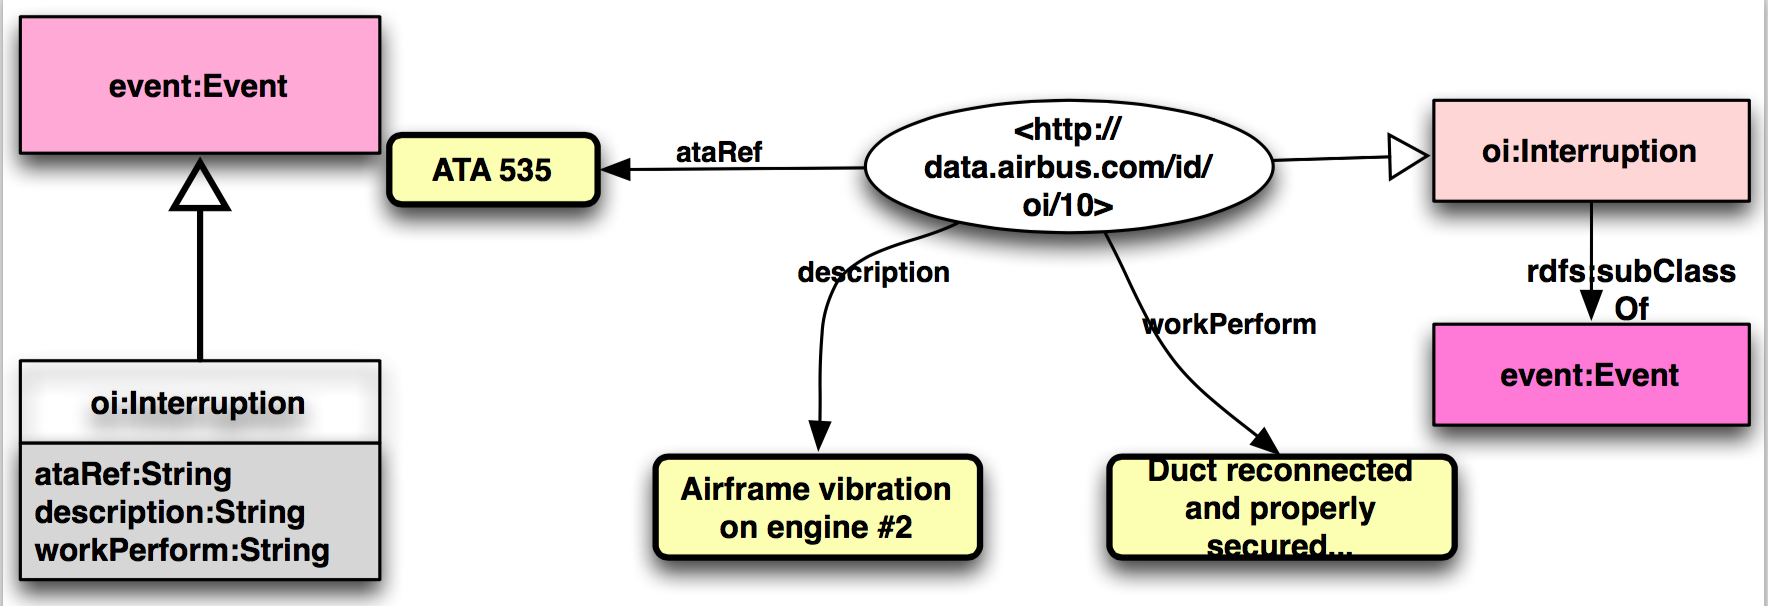
\includegraphics[scale=0.45]{img/oi-graph-model.png}
\caption{The left side shows the model and the right side an example of graph based on the OI vocabulary }
\label{figoi}
\end{figure} 
 

\subsection{Task vocabulary}
\label{sec:mpd-vocab} 
A vocabulary\footnote{\url{http://data.airbus.com/def/tf#}} for describing the relationships the failures and the maintenance tasks has been created to build a knowledge graph for integrating different silos of documents in Airbus organization. Currently, four main classes are defined: \textsf{tf:Task}, \textsf{tf:MRBR}, \textsf{tf:Failure} and \textsf{tf:ProgramTask}. Figure \ref{figtaskresource} shows an excerpt of the current usage of the vocabulary.   

\begin{figure}[!htb]
\centering
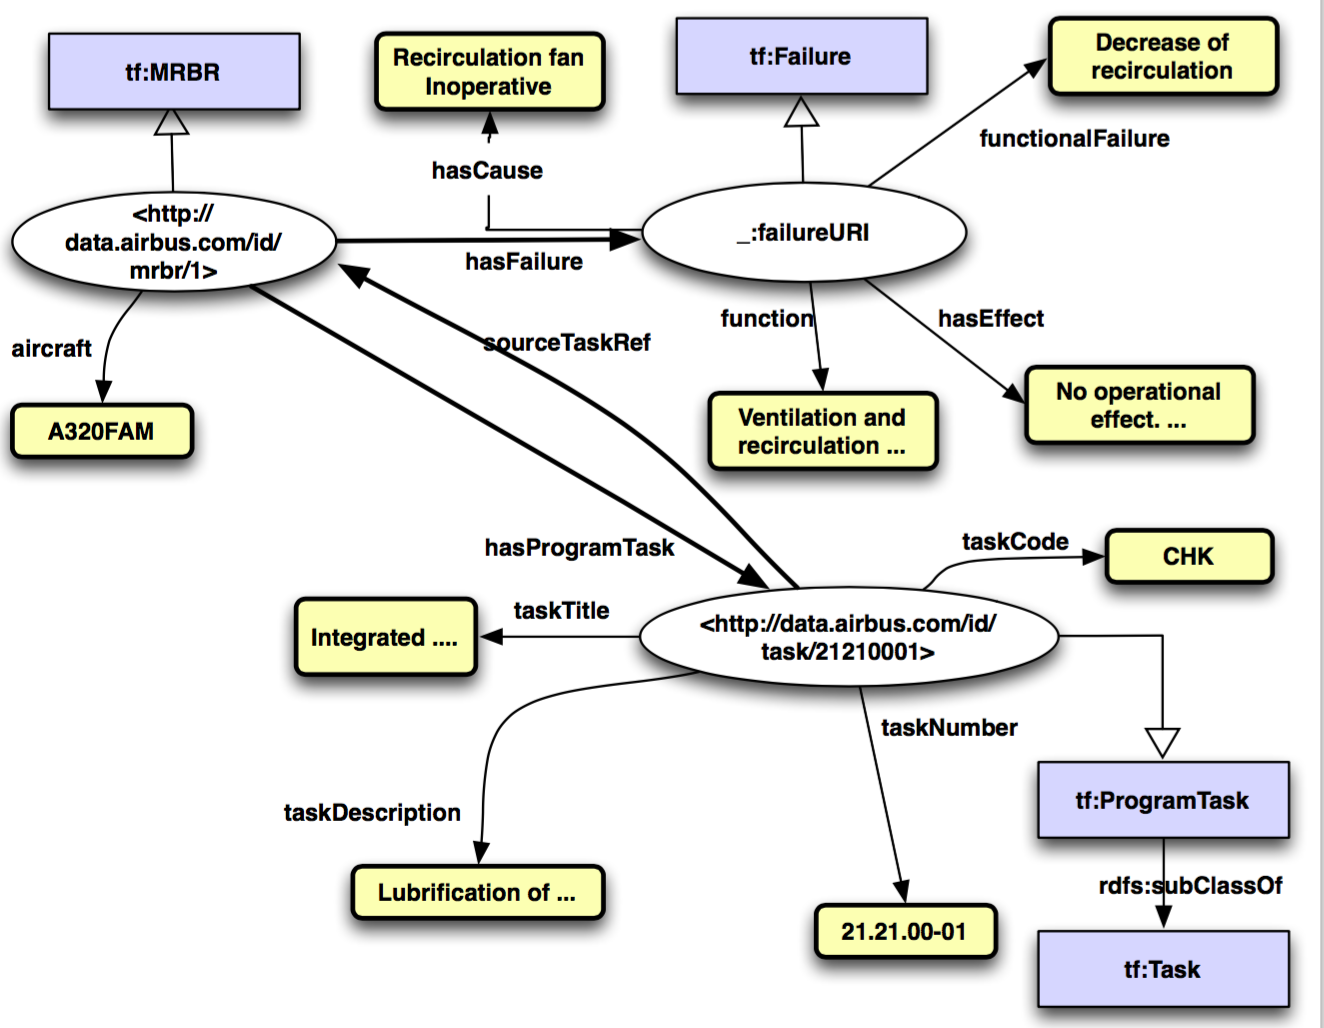
\includegraphics[scale=0.60]{img/task-mpd-graph.png}
\caption{A sample graph showing the relations between tasks, master documents and failures using the mpd-vocabulary.}
\label{figtaskresource}
\end{figure}


\section{RDF dataset}
\label{sec:a330rdf}
One of the main challenge in the generation of RDF data from the different spreadsheets is to create unique URIs to identify instances of the classes from the vocabularies. Each element of the graph should be identified uniquely with a persistent URI. The chosen scheme for the URI for generating RDF dataset is the following:
\textit{http://data.airbus.com/id/\{class\}/\{aircraft-family\}/\{year\}/\{code\}} \\
where \{class\} is one of (oi, task, mrbr) ; \{aircraft-family\} is one of (a330, a320) ; \{Year\} a four digit for the year and \{code\} is generated by concatenating a number of the XLS file name + raw number in the file. For example, this URI <\url{http://data.airbus.com/id/oi/a330/2014/07011231177}> represents in the Knowledge Graph the OI for an A330 received in 2014, where the description is within the file "isaim-a330-2014-0701to1231.xls", line 177. Table~\ref{tab:graphdata} shows the generated graphs in RDF for the two aircraft families: A330 and A320 for the period 2013 to 2015. 
The conversion process of the all the Excel files is performed by the Datalift~\cite{scharffe2012} platform, using custom CONSTRUCT SPARQL queries to transform columns to specific classes and properties.  

\begin{table}[!htb]
\centering
\begin{tabular}{|c|c|c||c|c|c|}

\hline 
Class & \multicolumn{2}{c||}{OI} & \multicolumn{3}{c|}{MRBR- MPD} \\ 
\hline 
Dataset & NbTriples & NbOIs & NbTriples & NbMRBR & NbTask \\ 
\hline 
A320 & 111,044 & 27,761 & 19,481 & 1,969 & 880 \\ 
\hline 
A330 & 60,867 & 21,400 & 54,457 & 6.871 & 4,234 \\ 
\hline  

\end{tabular} 
\caption{Overall number of the data converted into RDF by family of Aircraft for the period 2013-2014 for A330 and 2014-2015 for A320.}
\label{tab:graphdata}
\end{table}

\section{Semantic Annotation}
\label{sec:annotation}

Since the input of the descriptions and the work performed for the each OI is short text in English, an annotation pipeline based on the GATE architecture ~\cite{gatearch,kenter2005gate} is implemented to detect and tag the relevant concepts. CA-Manager is the annotation tool developed at Mondeca to annotate heterogeneous content with personalized pipelines based on GATE. 

\begin{figure}[!htb]
\centering
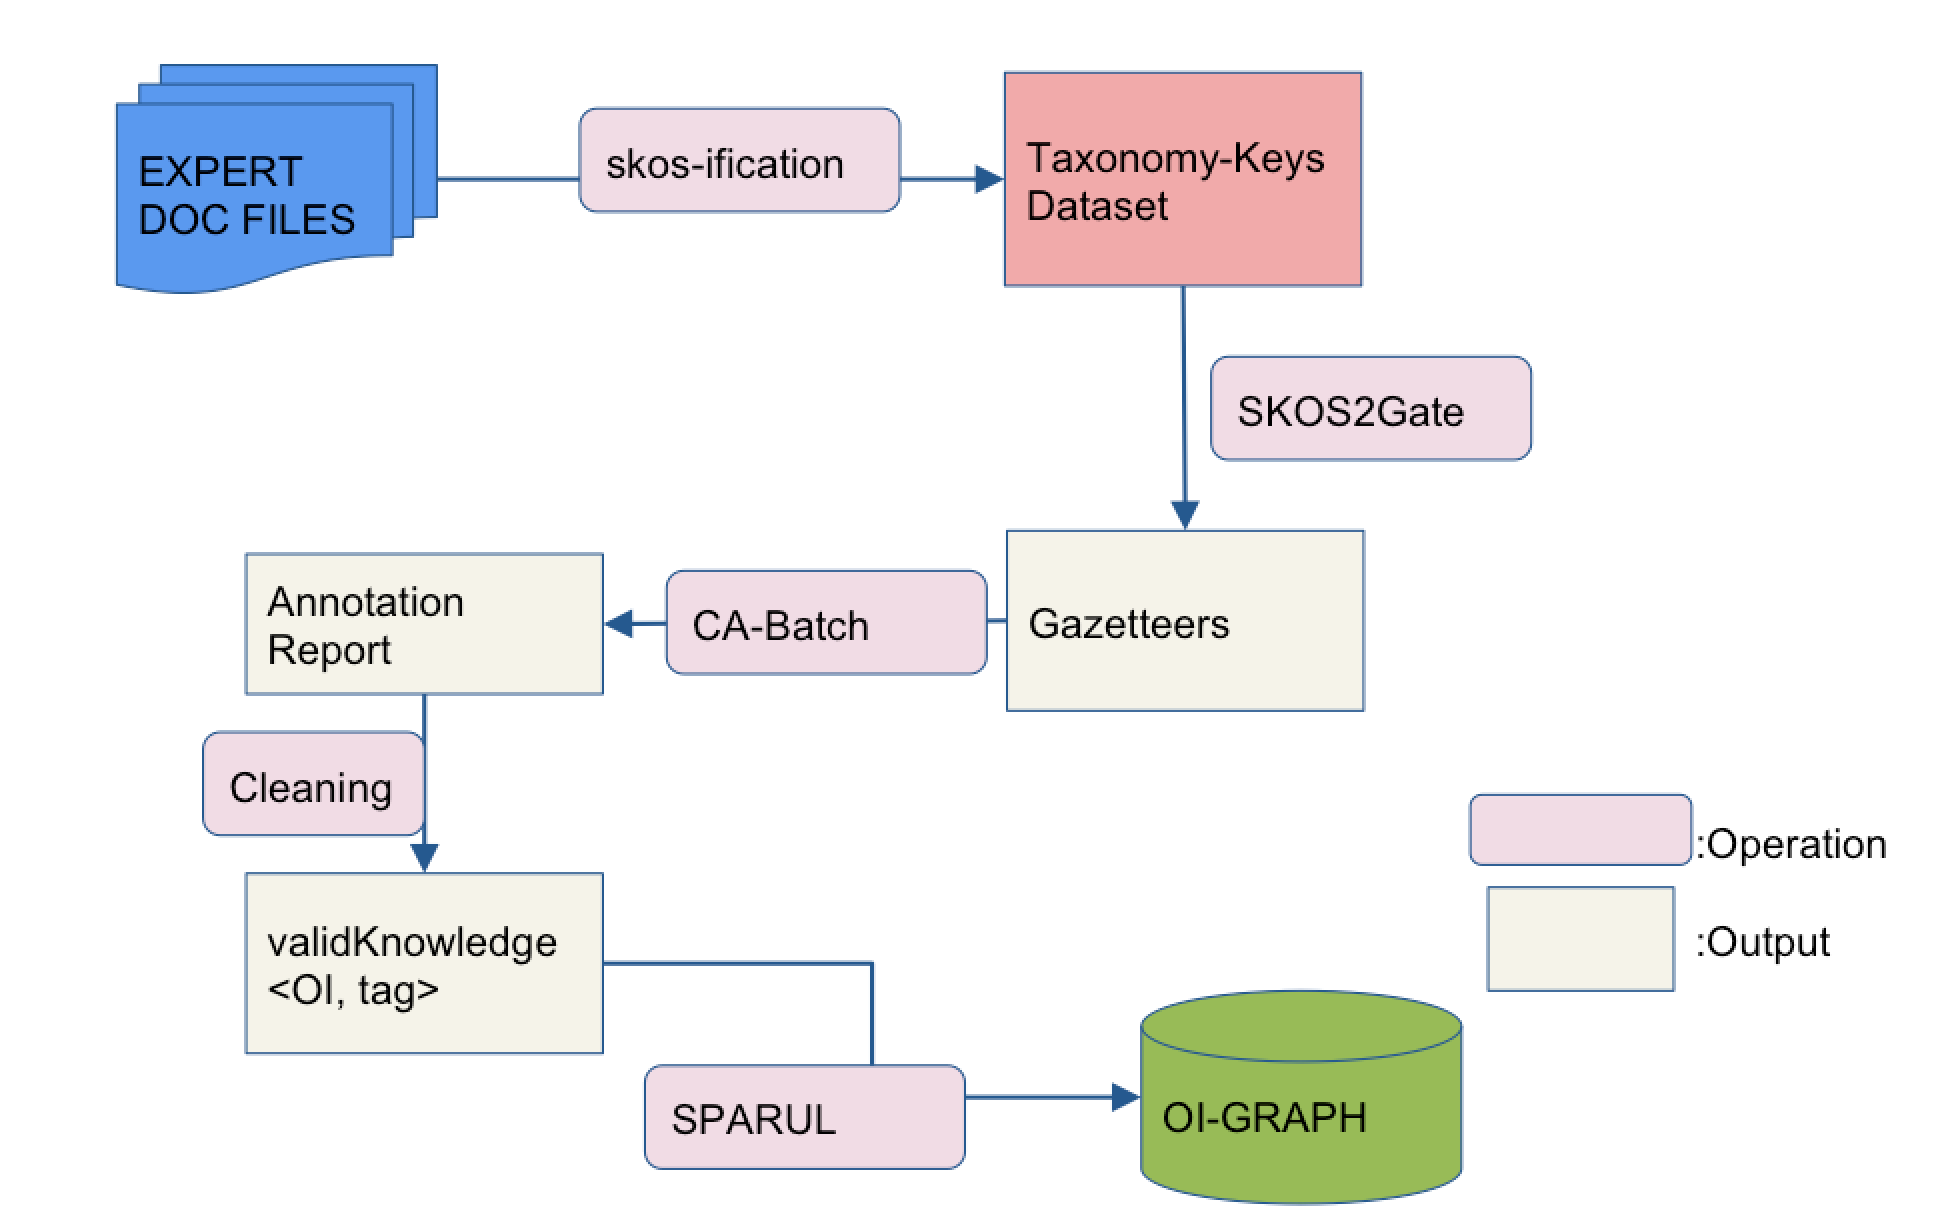
\includegraphics[scale=0.4]{img/archi-oi.png} 
\caption{Workflow of the semantic annotation and knowledge base updates.}
\label{figarchi}
\end{figure}

The architecture of the workflow consists of the following modules:
\begin{enumerate}
\item skos-ification module, in charge of converting into SKOS concepts the experts keywords.
\item SKOS2Gate module, for creating the gazetteer to be used during the annotation
\item CA-Batch module, for creating multi thread calls to annotate the text documents
\item Cleaning module, in charge of removing non relevant information from the reports generated by the annotator.
\item SPARUL module, which is in charge of updating the dataset in the endpoint using SPARQL updates queries.  
\end{enumerate}
 

\subsection{SKOS-ification Process}
\label{sec:skosification}

The skos-ification process consists of manually convert the keywords used by the expert of the domain into SKOS concepts that is later used for generating the gazetteers during the annotation. Since the input file are DOCX files, we manually create the RDF file in Turtle. Some rules and hypothesis are made during the process based on different interviews with the experts of the domain:

\begin{itemize}
\myitem Ordinal numbers such as ``Third'', ``First'', etc. are not taken into account. 
\myitem A keyword can not be at the same time in the description AND in the action work performed of the OI. The two sets are DISJOINTS.
\myitem Descriptors SHOULD be short concepts(names), with variants in the case of verbs that are treated as SYNONYMS (see sample below in Turtle format)
\myitem Expressions of type \textit{Not[properly][term]} are modeled as just [term a skos:Concept].
For e.g.,  in the case of the term ``not properly closed'', we only model the concept ``close'' with the variant closed. 
\end{itemize}


\begin{table}[h!tb]
\caption{Number of SKOS concepts manually generated from domain experts file, grouped by description and work performed.}
\label{tabskos}
\centering
\begin{tabular}{|c|c|c|c|c|c|}
%\caption{Number of SKOS concepts by types obtained after the skos-ification process.}
\hline 
Class & \multicolumn{2}{c|}{Description} & \multicolumn{2}{c|}{WorkPerformed} & Total  \\ 
\hline 
Feature & descItem & descAction & workItem & workAction & - \\ 
\hline 
SKOS concept & 47 & 45 & 22 & 16 & 130 \\ 
\hline 

\end{tabular} 

\end{table}
%include turtle sample starts here

\lstinputlisting[breaklines=true,language=turtle]{data/skos-sample.ttl}

\begin{figure}[!htb]
\centering
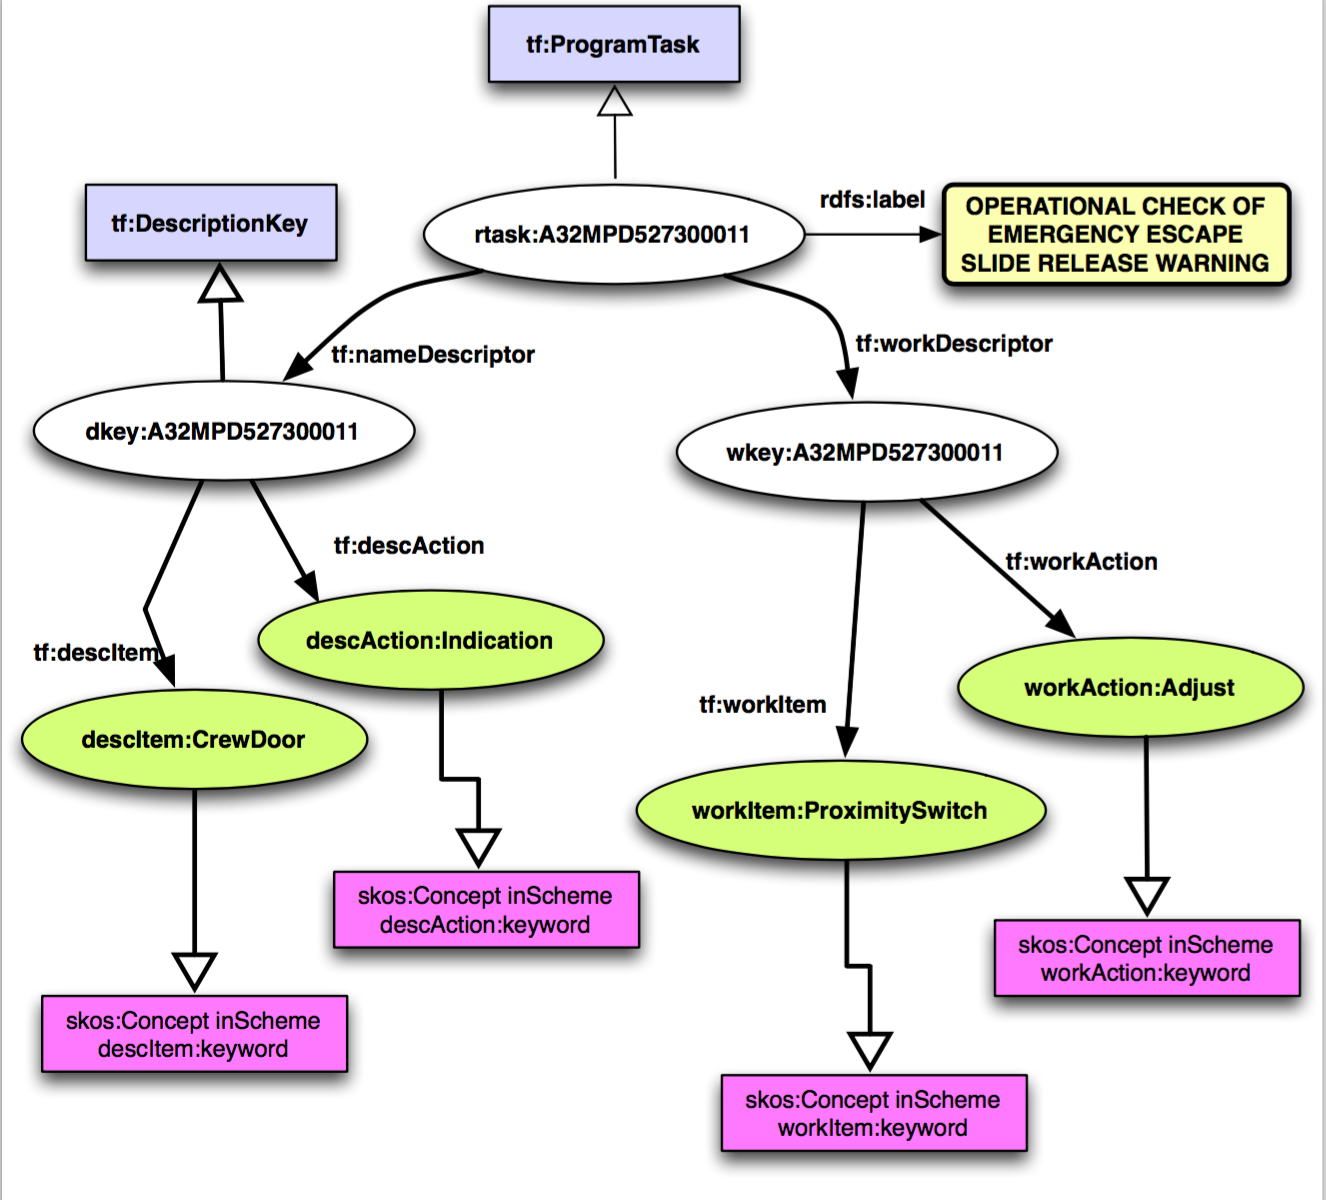
\includegraphics[scale=0.6]{img/descriptors_oi.png}
\caption{A sample of SKOS concepts used to model the experts' keywords  and linked to a task and maintenance graph}
\label{figdescriptors}
\end{figure}

The experiment described in this paper uses 20 tasks with keywords annotated manually by experts. Together with the corresponding task, the resulting file represents a gold standard where the descriptors are linked to appropriate task, as it is depicted in Figure \ref{figdescriptors}


The class \textsf{tf:DescriptionKey} is designed to capture the two different types of keywords: the description and the work performed. Once they are converted into SKOS concepts, they are used to identify relevant concepts in OIs text. Furthermore, four properties are used to link to the appropriate namespaces: \textsf{tf:descItem}, \textsf{tf:descAction}, \textsf{tf:workItem} and \textsf{tf:workAction}.


\subsection{Content Annotation}
\label{sec:contentannot}

The annotation process employed is based on a central component: the Content Augmentation Manager (CA-Manager)~\cite{cam2013}. The content augmentation manager (CA-Manager) is in charge of processing any type of content (plain text, XML, HTML, PDF, etc). This module extracts the concepts and entities detected using text mining techniques with the text input module. The strength of CA-Manager is to combine semantic technologies with a UIMA-based infrastructure\footnote{Unstructured Information Management Architecture (\url{http://uima.apache.org)}} which has been enriched and customized to address the specific needs of both semantic annotation and ontology population tasks.

\begin{figure}[!htb]
\centering
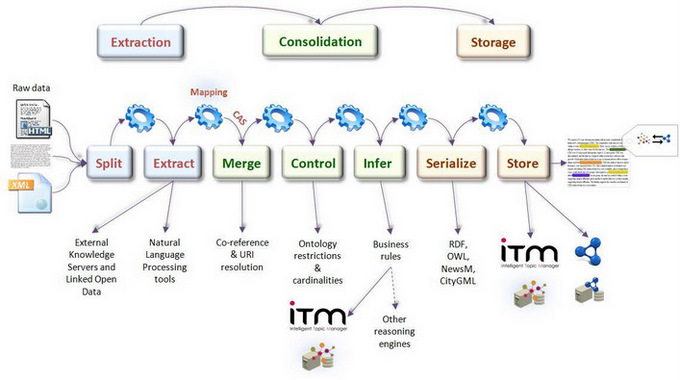
\includegraphics[scale=0.6]{img/cam_fig1.png}
\caption{Pipeline of annotation using CA-Manager}
\label{figcam}
\end{figure}


In the scenario presented in this paper, we use the GATE framework for the entity extraction. CA-Manager uses an ontology-based annotation schema to transform heterogeneous content (text, image, video, etc.) into semantically-driven and organized one. The overall architecture of CA-Manager is depicted in Figure~\ref{figcam}. 
We first create the gazetteer with the SKOS document obtained from the experts. We then launch in parallel 10  documents in multi-threads containing OIs. The annotation report contains the valid knowledge section, an RDF/XML document containing the URIs of the concepts detected by the annotator. We then use a python script to map each document with its corresponding URI. Finally, a SPARQL update query is launched to update the dataset containing the OI-Graph.   



\section{Graph Matching Algorithm}
\label{sec:matching}

\begin{algorithm}[h]\scriptsize
 \caption{GraphMatching (OI-Graph,MPD-Graph) - RLX Version}
\label{graphmatching}
\begin{algorithmic}[1]
\STATE Input: Set of OIs tagged  $<OI, tag>$ 
\STATE Input: Set of MPD in RDF with tags  $<MPD, tag>$.
\STATE INITIALIZE $Description = \{DescItems, DescActions\}$
\STATE INITIALIZE $WorkPerformed = \{WorkItems, WorkActions\} $
\STATE BEGIN
	\FOR {each $j \in MPD$}
		
		\STATE SELECT the list of tags in $DescActions$.
		\STATE FIND in the set $<OI, tag>$ with at least one $descItem$
		\STATE COMPUTE $P =$ card(OIs with at least one of the MPD tag in $DescActions$) = $|UnionOfDescActions|$
         		 
		\STATE SELECT the list of tags in $DescItems$.
	    \STATE FIND in the set $<OI, tag>$ with at least one $descAction$
		\STATE COMPUTE $Q =$ card(OIs with at least one of the MPD tag in $DescItems$) = $|UnionOfDescItems|$
		\STATE SELECT OIs in the set (P \textbf{OR} Q).
	    \STATE COMPUTE R = UNION(P,Q) = P + Q - INTERSECTION(P, Q) 
 	
 \ENDFOR	    		
	
	\FOR {each $j \in MPD$}
		
		\STATE SELECT the list of tags in $WorkActions$.
		\STATE FIND in the set $<OI, tag>$ with at \textit{least one} $workItem$
		\STATE COMPUTE $P' =$ card(OIs with at least one of the MPD tag in $WorkActions$) = $|UnionOfWorkActions|$
         		 
		\STATE SELECT the list of tags in $WorkItems$.
	    \STATE FIND in the set $<OI, tag>$ with at \textit{least one} $workAction$
		\STATE COMPUTE $Q' =$ card(OIs with at least one of the MPD tag in $WorkItems$) = $|UnionOfWorkItems|$
		\STATE SELECT OIs in the set (P' \textbf{OR} Q').
	    \STATE COMPUTE $R' = UNION(P',Q') = P' + Q' - INTERSECTION(P', Q') $
 	
 \ENDFOR	  
 
  \STATE SELECT OIs in the set $Description$ \textbf{OR} $WorkPerformed$.	
   \STATE COMPUTE $C =UNION(R, R’) = R + R’ - INTERSECTION (R, R’) $


    \RETURN $C$
  \STATE END
\end{algorithmic}
\end{algorithm}
 
Algorithm~\ref{graphmatching} (Relax version) is the first variant for creating candidates because of the lines 13, 23 and 26 of the algorithm, with the use the logical UNION operator to determining the intermediate sets for comparison and the resulting set of candidates in $C$. In this case, $C = UNION(P,Q,P',Q')$ where $P = UnionOfDescActions$, $Q = UnionOfDescItems$, $P' = UnionOfWorkActions$ and $Q' = UnionOfWorkItems$. All the queries used in the algorithm are based on SPARQL and the computation of the sets involving intersections make use of the LIMES~\cite{ngonga11} matching tool.  

A second approach for a less relax version (LRX-version) is to modify the lines 14, 24 and 27 respectively in Algorithm~\ref{graphmatching} by doing the adjustments described in Algorithm~\ref{graphmatching2}.


 
%%%%%%%%%%%%%%%%%%%%%%%%%
%%%  3. Experiments  %%%
%%%%%%%%%%%%%%%%%%%%%%%%%%

\section{Experiments and Results}
\label{sec:exp-results}

We perform experiments in both the annotation and the graph matching algorithm. To perform this, we use the datasets for the A330 family of Airbus aircrafts during the year 2013-2014.  

\subsection{Experiments}
We perform the annotation of $21,400$ OIs consisting of the descriptions and the work performed in English. We use a single machine on Windows 10, Core i7; 6 Go RAM. The annotation took 1h 48min (6434.464s), with an error rate by CA-Manager of 2.71\%. Moreover, 81.52\% of OIs were tagged (17,446), where more than 11K OIs have at least two tags. This is important because the graph matching algorithm uses this set of OIs with at least two tags detected. Table~\ref{tab:grapha330} gives more details of the annotation process results.  


\begin{algorithm}[!htb]\scriptsize
 \caption{GraphMatching - LRX-Version}
 \label{graphmatching2}
\begin{algorithmic}[1]
\STATE SAME INIT AS ALGO RLX-version \\
.....
\STATE BEGIN
 \STATE COMPUTE $R = UNION(P,P')$ \\
 ......
 \STATE COMPUTE $R' = UNION(Q,Q')$ \\
 ......
 \STATE COMPUTE $C = INTERSECTION(R, R’)$

\RETURN $C$
  \STATE END
\end{algorithmic}
\end{algorithm}

\begin{table}
\centering
\begin{tabular}{|c|c|c|}
\hline 
Graph & Feature & Number \\ 
\hline 
 \multirow{10}{*}{OI A330-Graph} & NbTriples & 60,867 \\ 
 
 & NbOI & 21,400 \\ 
 
 & NbOIs-tagged & 17,446\\ 
 
 & Max. tags & 12 \\ 
 
 & Min.tag & 1\\ 
 
 & NbOI-with-One-tag & 5,954 \\ 
 
 & CAM-processed & 20,819 \\ 
 
 & Errors-annotation & 581 \\ 
 
 & Time & 6,434.464s \\ 
\hline 
\end{tabular}
\caption{Details of the annotation content of the OIs for the A330 family.}
\label{tab:grapha330}
\end{table}
 
\subsection{Results}
\label{sec:results}

\begin{table}[!htp]
\scriptsize
\centering

\begin{tabular}{|c|c|c|c|c|c|c|c|c|c|c|} 
\hline 
Task ID & P & P' & Q & Q' & Inter(P,Q) & Inter(P',Q') & R=Union(P,Q) & R'=Union(P',Q') & Inter(R,R') & Union(R,R') \\ 
\hline 
MPD245000031 & 545 & 271 & 129 & 0 & 41 & 0 & 633 & 271 & 2 & \textbf{902}\\ 
\hline 
MPD271400031 & 110 & 306 & 0 & 366 & 0 & 250 & 110 & 422 & 7 & \textbf{525} \\ 
\hline 
MPD235100021 & 545 & 271 & 109 & 0 & 19 & 0 & 635 & 271 & 1 & \textbf{905} \\  
\hline 
\end{tabular} 
\caption{Results of the matching process in terms of size of the candidates using Algorithm~\ref{graphmatching} with three tasks for A330 and the OIs of the same aircraft family during the year 2013-2014.}
\label{tab:algo1}
\end{table}

In a more open criteria, as it is the case with algorithm~\ref{graphmatching}, we obtain the tasks T1(MPD245000031), T2 (MPD271400031) and T3 (MPD235100021) 902, 525 and 905 potential candidates. That means almost more than 95\% of the OIs are not relevant at all to those three tasks. But still many OIs to review by a human expert. So, after some interviews with the domain experts, the LRX-version of the algorithm (see Algorithm~\ref{graphmatching2}) is implemented suggesting a more reduced set of candidates, without loosing any good candidate. With this variant, it reduces significantly the number of the candidates (an average of 63\%) for reviewing.    

\begin{table}[!htp]
\scriptsize
\centering

\begin{tabular}{|c|c|c|c|c|c|c|c|c|c|c|} 
\hline 
Task ID & P & P' & Q & Q' & Inter(P,P') & Inter(Q,Q') & R=Union(P,P') & R'=Union(Q,Q') & Inter(R,R') \\ 
\hline 
MPD245000031 & 545 & 271 & 129 & 0 & 13 & 0 & 803 & 129 & \textbf{40}\\ 
\hline 
MPD271400031 & 110 & 306 & 0 & 366 & 8 & 0 & 408 & 366 & \textbf{4} \\ 
\hline 
MPD235100021 & 545 & 271 & 109 & 0 & 13 & 0 & 803 & 109 & \textbf{24} \\  
\hline 
\end{tabular} 
\caption{Results of the matching process when using Algorithm~\ref{graphmatching2}, the LRX version.}
\label{tab:algo2}
\end{table}


\section{Lessons Learned}
\label{sec:lessons}
One of the barrier in the adoption of Semantic technologies in industry is the difficulty to explain the key concepts underlying RDF model, vocabulary creation and the benefits of changing the paradigm from traditional data management to semantic repositories. This was one of the challenge of this project at Airbus, starting with a real use case to increasingly find the benefits of semantic technology to solve a real world problem. During the time frame of this work, several meetings where held to explain the `` why'' at every single steps. 

The team in charge of collecting the OIs from diverse companies and experts working on maintenance tasks has to progressively make a mental shift with the new paradigms introduced during this project:
\begin{itemize}
\xitem Data model by implementing vocabularies with Prot\'eg\'e~\cite{noy2001} from scratch driven by the existing data.
\xitem The notion of unique identifiers to be used across different data silos to represent the same real world object. Hence, a policy for creating persistent URIs was clearly identified as crucial
\xitem The confusion between the RDF model and the different serializations 
\end{itemize}  

This work also permits to identify many datasets that could be useful in other services at Airbus to bring more context. For example, during some interviews, the experts realized that some implicit knowledge can be derived actually from existing datasets, which otherwise are experts' experience. Moreover, the system proposed would not replace the experts but assist them in their work to speed up the process. This requirement 

Additionally, the conversion process into RDF reveals some errors in the legacy data. For example, sometimes there were not consistent use of the task code across different XLS files. This shows the benefits of our approach compared to existing one as it helps detecting and cleaning errors in the data.    

As the result of this work, the expert team is looking at a better combination for the output sets to adjust the proposed algorithm based on their evaluation of the proposed candidates. 
  


\section{Related Work}
\label{sec:soa}

This work falls under contributions and research in the intersection of natural language processing with GATE, enterprise semantic data management and matching techniques. The authors in~\cite{Uren200614} examine semantic annotation, identify a number of requirements, and review the generation of semantic annotation systems. 
Recently, in~\cite{andrews2012} it is defined a state of the art in semantic annotation models and a scheme that can be used to clarify requirements of end-user use cases. Moreover, the collection of real world applications from industry in~\cite{cardoso2007} tackle some challenges in the earlier adoption of semantic technologies in industry. Although some issues remind challenging today, a diversity of domains applying semantics is visible worldwide. To the best of our knowledge, this paper is the first applying semantics in aircraft industry.  



%%%%%%%%%%%%%%%%%%%%%%%%%%%%%%%%%%%%%%%
%%%  4. Conclusion and Future Work  %%%
%%%%%%%%%%%%%%%%%%%%%%%%%%%%%%%%%%%%%%%

\section{Conclusion and Future Work}
\label{sec:conclusion}
This paper presents a semi-automatic approach using semantic technologies to assist the experts of the aircraft domain to improve the matching process of Operational Interruptions with related Maintenance Programming Task. Our approach combines text annotation using GATE alike system for annotation and a graph matching algorithm for suggesting candidates. Annotation of 21,400 OIs show a high amount of tag detected (82\%) with a small amount of expert concepts. The graph matching technique shows that by combining suitable combinations, it is possible to reduce to up to 63\% the amount of candidates of OIs to be assessed by domain experts. The first results shed the light for future intensive application of semantic technologies at Airbus for many other aspects, such as data integration, data fusion and semantic recommendation tools. 

For future work, we plan to improve the semantic annotation by looking at the better management of noises in the text for annotation. Also, we plan to implement fuzzy annotation in the GATE pipeline to find a trade-off between performance and recall. Currently we are using a small gazetteer, we plan to integrate external sources to have a much bigger scope for the terms to detect.  



%%%%%%%%%%%%%%%%%%%%%%%%%
%%%  Acknowledgments  %%%
%%%%%%%%%%%%%%%%%%%%%%%%%

\paragraph{\textbf{Acknowledgments.}} %\label{sec:acknowledgments}
We would like to thank the Airbus team in Toulouse and ATOS colleagues for their valuable input and partnership.

\bibliographystyle{abbrv}
%\nocite{*}
\bibliography{iswc2016}
\end{document}
